\documentclass{article}\usepackage[]{graphicx}\usepackage[]{xcolor}
% maxwidth is the original width if it is less than linewidth
% otherwise use linewidth (to make sure the graphics do not exceed the margin)
\makeatletter
\def\maxwidth{ %
  \ifdim\Gin@nat@width>\linewidth
    \linewidth
  \else
    \Gin@nat@width
  \fi
}
\makeatother

\definecolor{fgcolor}{rgb}{0.345, 0.345, 0.345}
\newcommand{\hlnum}[1]{\textcolor[rgb]{0.686,0.059,0.569}{#1}}%
\newcommand{\hlsng}[1]{\textcolor[rgb]{0.192,0.494,0.8}{#1}}%
\newcommand{\hlcom}[1]{\textcolor[rgb]{0.678,0.584,0.686}{\textit{#1}}}%
\newcommand{\hlopt}[1]{\textcolor[rgb]{0,0,0}{#1}}%
\newcommand{\hldef}[1]{\textcolor[rgb]{0.345,0.345,0.345}{#1}}%
\newcommand{\hlkwa}[1]{\textcolor[rgb]{0.161,0.373,0.58}{\textbf{#1}}}%
\newcommand{\hlkwb}[1]{\textcolor[rgb]{0.69,0.353,0.396}{#1}}%
\newcommand{\hlkwc}[1]{\textcolor[rgb]{0.333,0.667,0.333}{#1}}%
\newcommand{\hlkwd}[1]{\textcolor[rgb]{0.737,0.353,0.396}{\textbf{#1}}}%
\let\hlipl\hlkwb

\usepackage{framed}
\makeatletter
\newenvironment{kframe}{%
 \def\at@end@of@kframe{}%
 \ifinner\ifhmode%
  \def\at@end@of@kframe{\end{minipage}}%
  \begin{minipage}{\columnwidth}%
 \fi\fi%
 \def\FrameCommand##1{\hskip\@totalleftmargin \hskip-\fboxsep
 \colorbox{shadecolor}{##1}\hskip-\fboxsep
     % There is no \\@totalrightmargin, so:
     \hskip-\linewidth \hskip-\@totalleftmargin \hskip\columnwidth}%
 \MakeFramed {\advance\hsize-\width
   \@totalleftmargin\z@ \linewidth\hsize
   \@setminipage}}%
 {\par\unskip\endMakeFramed%
 \at@end@of@kframe}
\makeatother

\definecolor{shadecolor}{rgb}{.97, .97, .97}
\definecolor{messagecolor}{rgb}{0, 0, 0}
\definecolor{warningcolor}{rgb}{1, 0, 1}
\definecolor{errorcolor}{rgb}{1, 0, 0}
\newenvironment{knitrout}{}{} % an empty environment to be redefined in TeX

\usepackage{alltt}
\usepackage{amsmath} %This allows me to use the align functionality.
                     %If you find yourself trying to replicate
                     %something you found online, ensure you're
                     %loading the necessary packages!
\usepackage{amsfonts}%Math font
\usepackage{graphicx}%For including graphics
\usepackage{hyperref}%For Hyperlinks
\usepackage[shortlabels]{enumitem}% For enumerated lists with labels specified
                                  % We had to run tlmgr_install("enumitem") in R
\hypersetup{colorlinks = true,citecolor=black} %set citations to have black (not green) color
\usepackage{natbib}        %For the bibliography
\setlength{\bibsep}{0pt plus 0.3ex}
\bibliographystyle{apalike}%For the bibliography
\usepackage[margin=0.50in]{geometry}
\usepackage{float}
\usepackage{multicol}

%fix for figures
\usepackage{caption}
\newenvironment{Figure}
  {\par\medskip\noindent\minipage{\linewidth}}
  {\endminipage\par\medskip}
\IfFileExists{upquote.sty}{\usepackage{upquote}}{}
\begin{document}

\vspace{-1in}
\title{Lab 7 and 8 -- MATH 240 -- Computational Statistics}

\author{
  Jack Schaeffer \\
  Math 240  \\
  Professor Cipolli  \\
  {\tt jschaeffer@colgate.edu}
}

\date{April 1, 2025}

\maketitle

\begin{multicols}{2}
\begin{abstract}
This lab is an overview of the beta distribution including potential uses and examples. Further examination of the distribution includes analysis of statistic summaries, the effect of sample size, and point estimator methods.
\end{abstract}

\noindent \textbf{Keywords:} Beta distribution; point estimators; moments of distribution

\section{Introduction}

The beta distribution is a continuous distribution that models a variable X that has values within [0,1]. The shape and properties of the beta distribution are reliant on the parameters $\alpha$ and $\beta$ ($\alpha>0$, $\beta>0$).

My initial work was focused on the effect that $\alpha$ and $\beta$ have on the distribution before moving into analysis of statistical properties and point estimators. This work included testing sample size's importance in producing accurate data and application of the beta distribution to model death rates in 2022.

\section{Density Functions and Parameters}

Due to the beta distribution's separate shape parameters $\alpha$ and $\beta$, the distribution can have very different appearances and statistical properties depending on parameter values.





% latex table generated in R 4.4.2 by xtable 1.8-4 package
% Tue Apr  1 12:13:33 2025
\begin{table}[H]
\centering
\begingroup\small
\begin{tabular}{lrrrr}
  \hline
Values & Mean & Variance & Skew & Kurtosis \\ 
  \hline
Alpha = 2, Beta = 5 & 0.29 & 0.03 & 0.60 & -0.12 \\ 
  Alpha = 5, Beta = 5 & 0.50 & 0.02 & 0.00 & -0.46 \\ 
  Alpha = 5, Beta = 2 & 0.71 & 0.03 & -0.60 & -0.12 \\ 
  Alpha = 0.5, Beta = 0.5 & 0.50 & 0.12 & 0.00 & -1.50 \\ 
   \hline
\end{tabular}
\endgroup
\caption{Properties in comparison to differing parameter values} 
\label{distrib.tab}
\end{table}



\begin{figure}[H]
 \begin{center}
 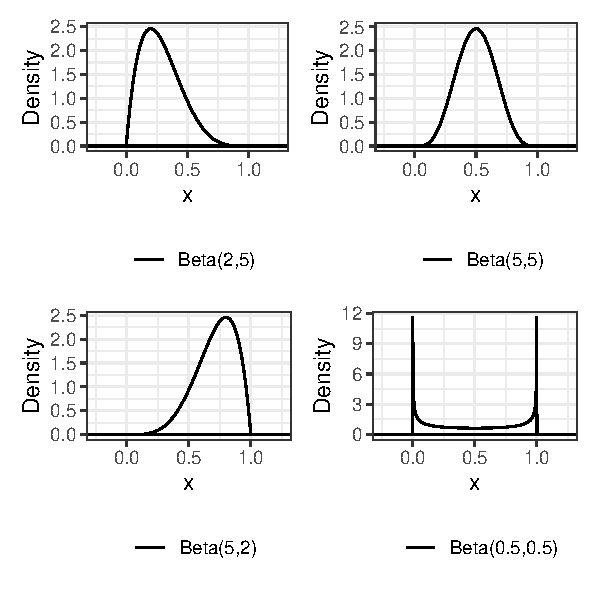
\includegraphics[scale=0.75]{parameter_comparison.pdf}
 \caption{Density plots of the beta distribution with differing parameter values}
 \label{fig1}
 \end{center}
 \end{figure}




Figure \ref{fig1} showcases the noticeable difference in the shape of the beta distribution depending on parameter values. These differences are reflected in the plots' properties in Table \ref{distrib.tab}. 


\section{Properties}
As is clearly shown from Figure \ref{fig1} and Table \ref{distrib.tab}, both the beta distribution's shape and characteristics are dependent on $\alpha$ and $\beta$. The population-level characteristics can be calculated by

\begin{align*}
E(X) &= \frac{\alpha}{\alpha + \beta} \tag{The Mean} \\
var(X) &= \frac{\alpha\beta}{(\alpha + \beta)^2(\alpha + \beta + 1)} \tag{The variance} \\
skew(X) &= \frac{2(\beta-\alpha)\sqrt{\alpha + \beta + 1}}{(\alpha + \beta + 2)\sqrt{\alpha\beta}} \tag{The Skewness} \\
kurt(X) &= \frac{6[(\alpha-\beta)^2(\alpha+\beta+1)-\alpha\beta(\alpha+\beta+2)]}{\alpha\beta(\alpha+\beta+2)(\alpha+\beta+3)} \tag{The Excess Kurtosis}
\end{align*}

The above equations are reflective of the answers seen in Table \ref{distrib.tab}. For example, when $\alpha$ and $\beta$ are equal, the skewness is always equal to zero.

\section{Estimators}
When the exact parameters of a beta distribution are unknown, we have to instead rely on data samples to estimate the distribution. To estimate population-level characteristics, we can use moments of distribution. The $k$th uncentered moment of distribution is 

\[E(X^k) = \int_\chi x^kf_X(x)dx,\]

while the $k$th centered moment of distribution is

\[E[(X-\mu_X)^k] = \int_\chi (x-\mu_X)^kf_X(x)dx.\]

Using these moments, we can calculate the population-level characteristics as

\begin{align*}
\mu_X = E(X) & \tag{The Mean} \\ 
\sigma^2_X = var(X) &= E[(X-\mu_X)^2] \tag{The Variance} \\
skew(X) &= \frac{E[(X-\mu_X)^3]}{E[(X-\mu_X)^2]^{3/2}} \tag{The Skewness} \\
kurt(X) &= \frac{E[(X-\mu_X)^4]}{E[(X-\mu_X)^2]^2}-3 \tag{The Excess Kurtosis}
\end{align*}

To test the accuracy of data sampling compared to population-level values, we can overlay the population-level density plot over a histogram of sampled data ($n=500$).

\begin{figure}[H]
 \begin{center}
 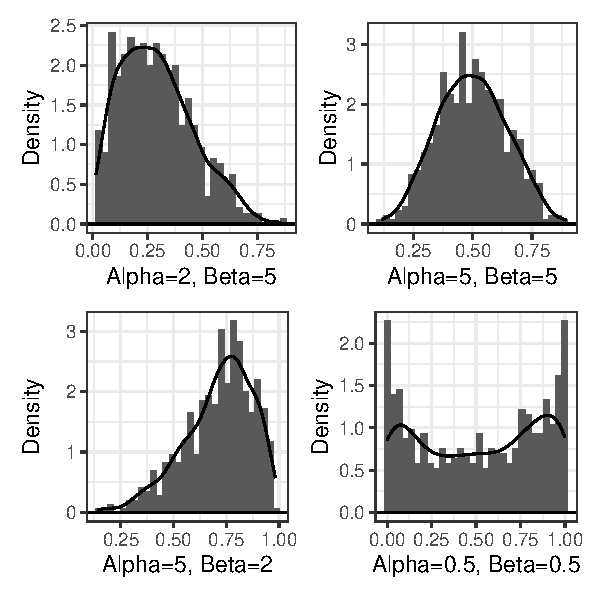
\includegraphics[scale=0.75]{density_histogram.pdf}
 \caption{Comparison of estimator versus population-level values}
 \label{fig2}
 \end{center}
 \end{figure}





% latex table generated in R 4.4.2 by xtable 1.8-4 package
% Tue Apr  1 12:13:53 2025
\begin{table}[H]
\centering
\begingroup\small
\begin{tabular}{lrrrr}
  \hline
Variable & Mean & Variance & Skewness & Kurtosis \\ 
  \hline
Alpha = 2, Beta = 5 & 0.29 & 0.03 & 0.57 & 2.78 \\ 
  Alpha = 5, Beta = 5 & 0.50 & 0.02 & 0.06 & 2.54 \\ 
  Alpha = 5, Beta = 2 & 0.71 & 0.03 & -0.74 & 3.22 \\ 
  Alpha = 0.5, Beta = 0.5 & 0.52 & 0.12 & -0.11 & 1.55 \\ 
   \hline
\end{tabular}
\endgroup
\caption{Estimated characteristics of the beta distribution for specified parameters} 
\label{estim.tab}
\end{table}


Both Figure \ref{fig2} and Table \ref{estim.tab} demonstrate the effectiveness of using an estimator as they produce results similar to the population-level values. However, we later considered how strong of an effect sample size had on the estimator's effectiveness. Using \texttt{cumstats}, I generated Figure \ref{fig3} as estimations of distribution characteristics as sample size increased \citep{cumstats}. Figure \ref{fig4} demonstrates the distribution of estimated characteristics when $n=500$ for different data samples.

\begin{figure}[H]
 \begin{center}
 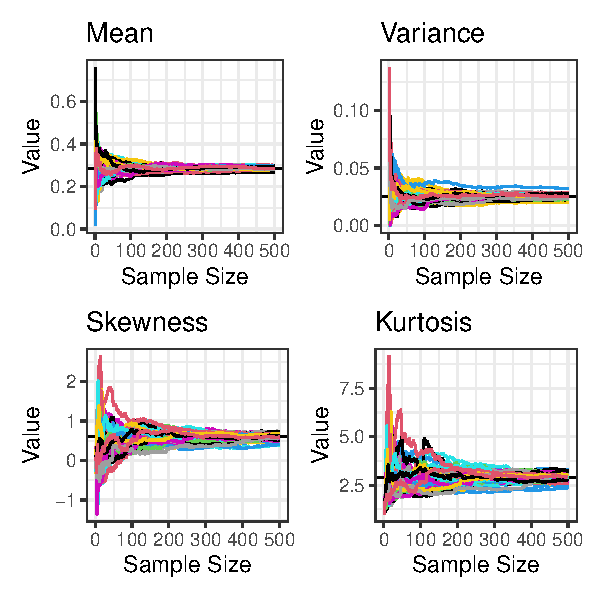
\includegraphics[scale=0.7]{sample_comparison.pdf}
 \caption{Cumulative characteristic values}
 \label{fig3}
 \end{center}
 \end{figure}

\begin{figure}[H]
 \begin{center}
 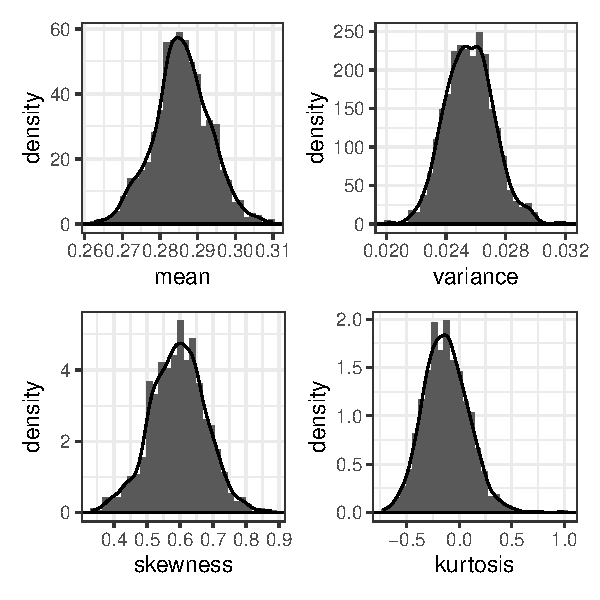
\includegraphics[scale=0.7]{sampling_distrib.pdf}
 \caption{Histogram of characteristic values}
 \label{fig4}
 \end{center}
 \end{figure}

In Figure \ref{fig3}, the values are extremely inconsistent for low sample values, which changed considerably on each calculation. As sample size increases, however, the values converge towards the population-level value indicated by the horizontal black line, demonstrating that having a large enough sample size is important for producing reliable data. At this high sample size, we can see that property values stay similar through differing data samples.




\section{Example: Death Rates Data}
To demonstrate the beta distribution's use in real life, I used data from the World Bank on death rates in 2022. 

%%%%%%%%%%%%%%%%%%%%%%%%%%%%%%%%%%%%%%%%%%%%%%%%%%%%%%%%%%%%%%%%%%%%%%%%%%%%%%%%
% Bibliography
%%%%%%%%%%%%%%%%%%%%%%%%%%%%%%%%%%%%%%%%%%%%%%%%%%%%%%%%%%%%%%%%%%%%%%%%%%%%%%%%
\vspace{2em}

\noindent\textbf{Bibliography:} Note that when you add citations to your bib.bib file \emph{and}
you cite them in your document, the bibliography section will automatically populate here.

\begin{tiny}
\bibliography{bib}
\end{tiny}
\end{multicols}

%%%%%%%%%%%%%%%%%%%%%%%%%%%%%%%%%%%%%%%%%%%%%%%%%%%%%%%%%%%%%%%%%%%%%%%%%%%%%%%%
% Appendix
%%%%%%%%%%%%%%%%%%%%%%%%%%%%%%%%%%%%%%%%%%%%%%%%%%%%%%%%%%%%%%%%%%%%%%%%%%%%%%%%
\newpage
\onecolumn
\section{Appendix}

If you have anything extra, you can add it here in the appendix. This can include images or tables that don't work well in the two-page setup, code snippets you might want to share, etc.

\end{document}
